\section{Procedure and setup}

\subsection{Measuring the band gap}
In this part of the experiment, we will measure the absorption and 
transmission of the two sample of Si and Ge, respectively. 
Both quantities are measured with an underlying spectrum of a lamp, 
partitioned into its components by an optical gratings mounted 
on a rotating disk. The angle of the grating towards the beam 
path determines the wavelength of incident light at the sample. 
From the setup sketched in figure \ref{fig:setup_band_gap} 
and the diffraction condition of the grating, one can obtain the following 
relation between energy $E$ of the incoming photons, and angle 
$\phi$:
\begin{equation}
    E(\phi) = \frac{h c}{2d |\sin(\phi)| \cos(\psi)}
    \label{eq:E_g}
\end{equation}
with the half aperture angle of the optical table $\psi$ and lattice 
constant $d$. $h$ and $c$ are Planck's constant and the speed of 
light in vacuum, respectively. The semiconductor is connected 
to a voltage source in order to measured th signal. 
The signal-to-noise ratio is increased by a lock-in amplifier. A chopper 
in front of the lamp creates rectangularly distributed intensities, 
which coincide with the signals measured at the semiconductor 
and the pyrodetector (on the time scale of the chopper 
    both sensors register instantaneously). 
The integrated signal is processed by a computer, which also
perceives information about the angle of the grating. 
All signals are put out in one file and graphically, showing absorption 
and transmission over angle or energy (the energy is readily computed). 

\begin{figure}
    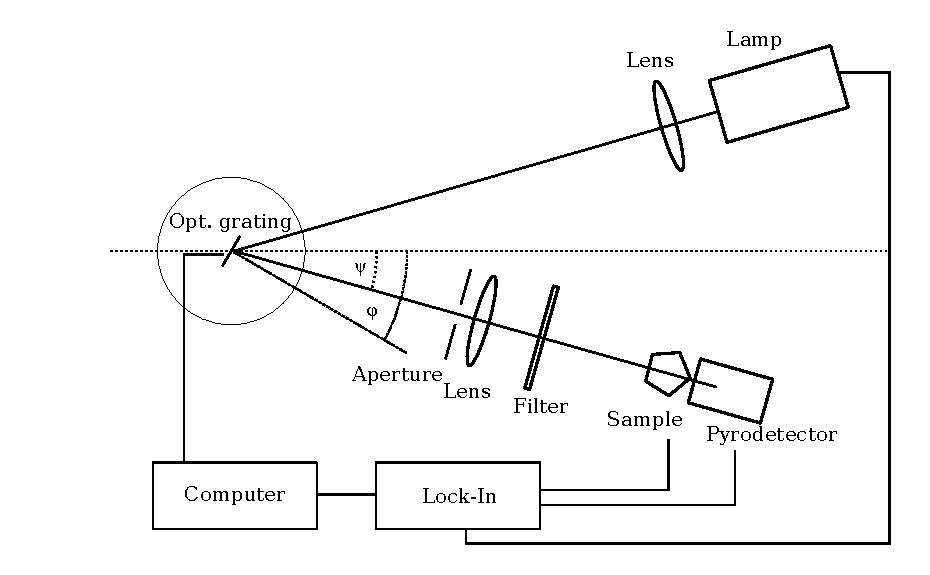
\includegraphics[width=\textwidth]{figures/setup_band_gap}
    \caption{
        Sketch of the experimental setup for the measurement of 
        absorption and transmission spectrum of semiconductors, 
        defining the angles $\psi$ and $\phi$.
        }
    \label{fig:setup_band_gap}
\end{figure}

The setup for us is fairly simple, since most of the bank and 
electronics are already installed and connected. 
The beam path is calibrated such that 
the light emitted by the lamp reaches the grating as a parallel bundle
(the distance lamp -- lens $l_1$ must equal the focal length $f_{l_1}$ of $l_1$).
The second lens has to be adjusted such that that light is focused onto 
the pyrodetector. After adding the grating, the measured angle has to be 
calibrated, setting $0^\circ$ for the case of reflected light being centered 
on the aperture. The filter is added between lens and detector. Both 
filter and grating are chosen according to the sample semiconductor 
examined. Finally, the sample is put on the pyrodetector. 

The following four measurements are done:
\begin{itemize}
    \item
        Transmission and absorption (simultaneously) over the entire 
        semicircle;
    \item
        Background for both transmission and absorption, measured by 
        closing the aperture;
    \item
        Spectrum of the lamp with filter, measured without the sample;
    \item
        Approximation of errors by measuring the intensity at one angle 
        repeatedly.
\end{itemize}
For the evaluation,use the fact, that for photons of
$E_\gamma = E_g$, absorption and transmission are equally probable. 
We can thus measure this energy by finding the intersection 
of both signals normalized. The individual steps to be taken are 
the following:
\begin{itemize}
    \item
        We correct for the background and normalize to the spectrum of 
        the light source by 
        \begin{align}
            T_\mathrm{real} &= \frac{T_\mathrm{measured} - 
                T_\mathrm{background}}{L} 
            \label{eq:t_real} \\
            A_\mathrm{real} &= \frac{A_\mathrm{measured} - 
                A_\mathrm{background}}{L} \, .
            \label{eq:a_real}
        \end{align}
        $T$ and $A$ refer to transmission and absorption signals respectively. 
        $L$ is the spectrum of the lamp with filter, to which we normalize.
        The units of the measured quantities on the right side are those 
        of the lock-in amplifier. We are, however, only interested in relative 
        coefficients, represented by the left hand side quantities. 
    \item
        We perform a linear fit on the flanks of both curves. Both 
        curves are now intersected by horizontal lines going through the 
        maximum of transmission and the minimum of absorption. 
        These intersects give boundaries for $E_g$, which 
        is simply approximated by the mean of these boundaries. 
\end{itemize}


\subsection{The Haynes \& Shockley experiment}
In the Haynes and Shockley experiment, we visualize the movement 
of electrons and a semiconductor and use the measured 
charge distribution to extract three characteristic 
properties of the examined germanium sample.
An overview of the concept of the experiment is given 
in figure \ref{fig:H_S_overview}
A laser beam lifts a cloud of electrons from the valence band into 
conducting band at one end of the sample. 
These free electrons are accelerated 
by an electric fields created with the voltage $U_\mathrm{acc}$ 
applied between the two ends of the sample. 
At a distance $d$ away from the laser, a needle 
registers the charge density in a linear fashion.
This signal is visualized on the oscilloscope, which
is triggered externally by a signal from the pulse 
generator. 
Both $d$ and $U_\mathrm{acc}$ can be variated. 
The laser beam is applied only during 3 \% of the time, in 
order to prevent the semiconductor from heating up. 

\begin{figure}
    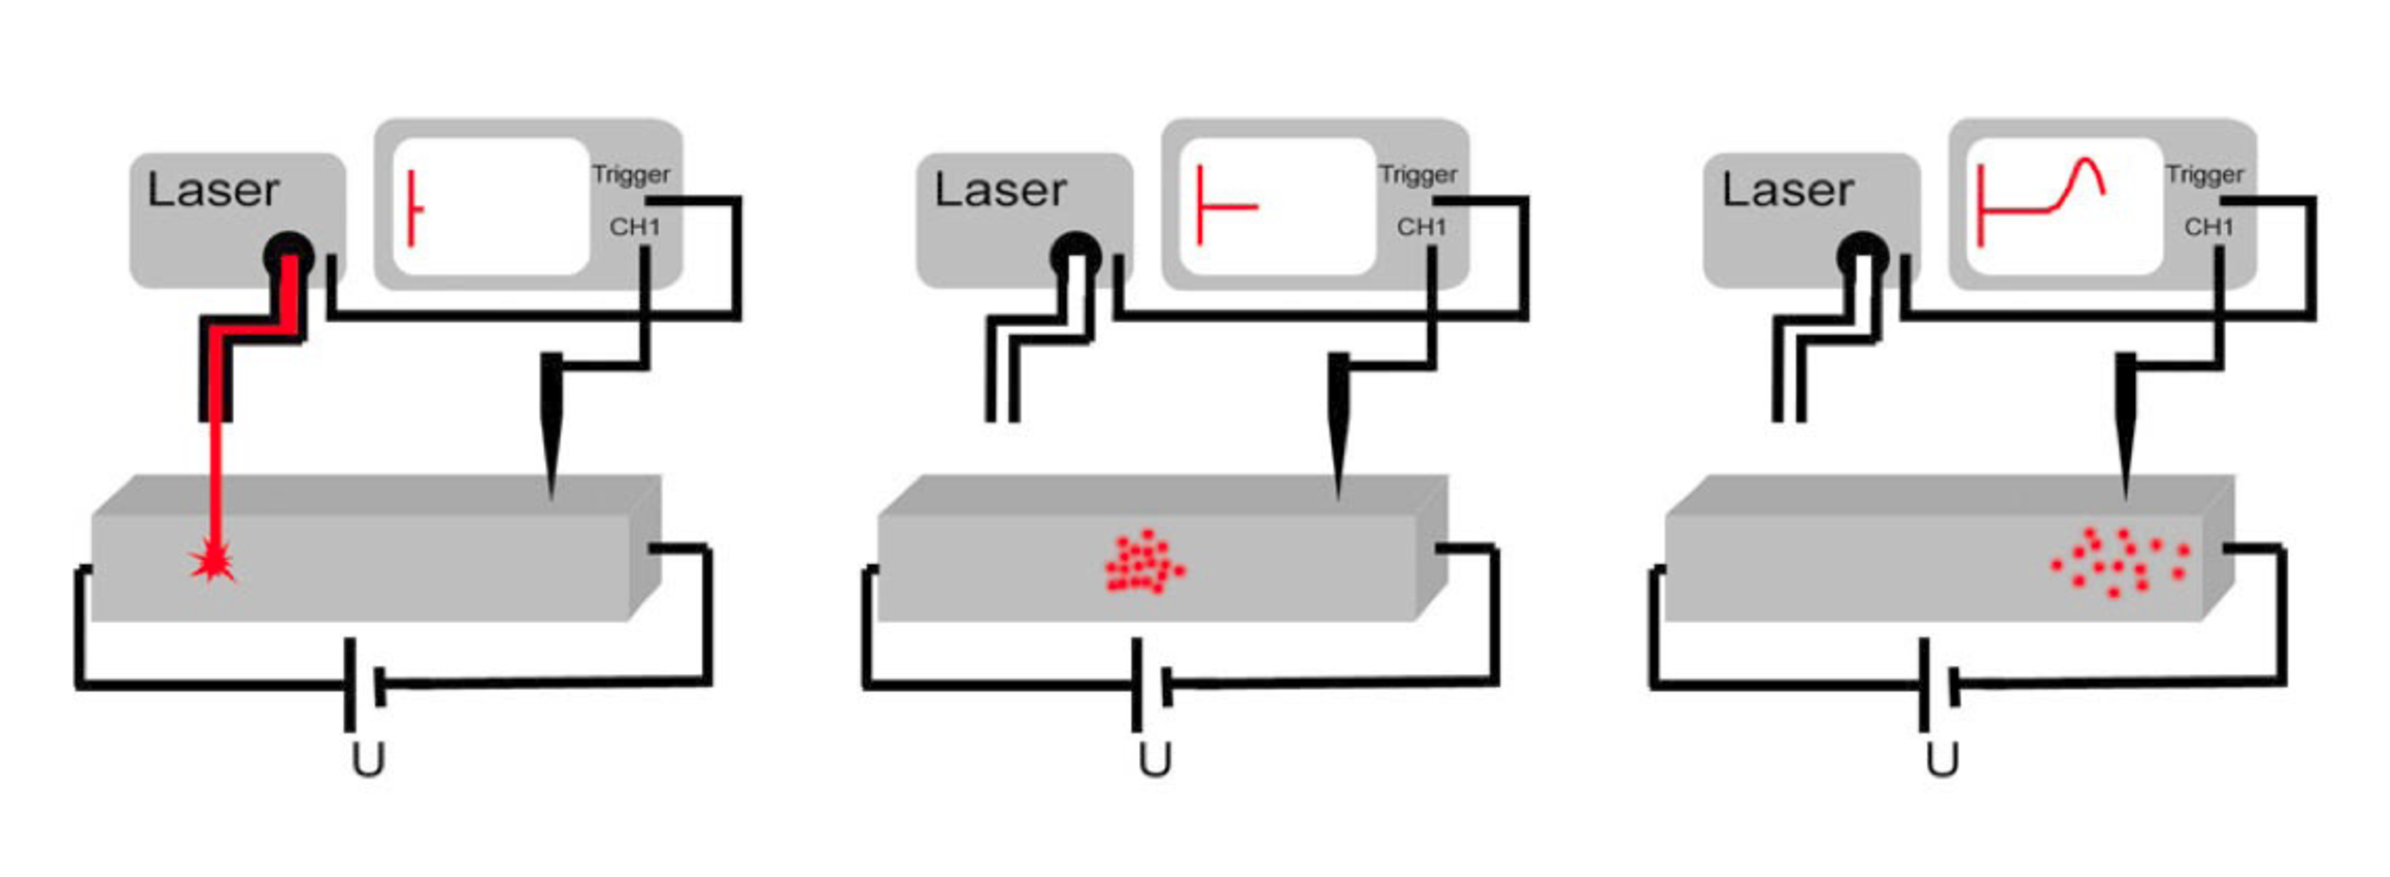
\includegraphics[width=\textwidth]{figures/H_S_overview}
    \caption{
        Concept of the Haynes and Shockley experiment. 
        Each figure visualizes a step in time from 
        generating the free charges by inserting a laser pulse 
        to registering the charge density variation "flying by" 
        the needle. $U$ is the applied acceleration voltage. 
        Taken from~\cite{ver}.
        }
    \label{fig:H_S_overview}
\end{figure}

By fitting gaussians of the form 
\begin{equation}
    c(x) = A \cdot \frac{1}{\sqrt{2 \pi \sigma^2}} 
    \cdot \exp\left( -\frac{1}{2}\frac{\left( x - x_c \right)^2}{\sigma^2} \right)
    \label{eq:gaussian}
\end{equation}
on the obtained data, we get the following 
correspondences, as described in the theory section~\ref{eq:c_t_x}: 
\begin{itemize}
    \item
        mobility of free electrons $\mu_n$ -- 
        center of distribution $x_c$
        \begin{equation}
            x_c(t) = \mu_n E t
        \end{equation}
    \item
        life time of electrons $\tau_n$ --
        amplitude $A(t)$
        \begin{equation}
            A(t) = C \exp\left(-\frac{t}{\tau_n}\right)
        \end{equation}
    \item
        diffusion constant $D_n$ --
        variance $\sigma^2$
        \begin{equation}
            \sigma^2(t) = 2 D_n t
        \end{equation}
\end{itemize}

\subsection{Semiconductor detectors}
Here, the suitability of semiconductors as detectors for 
ionizing rays is demonstrated on the basis of a silicon 
and a cadmium telluride semiconductor. We will record 
the spectra of $^{57}$Co and $^{241}$Am with both detectors 
each. 
The setup is shown in figure \ref{fig:setup_detector}.
The semiconductor is
locked onto a circuit board with preamplifier and shaping 
amplifier which amplify the signal linearly to the energy 
absorbed in the detector. 
These electronics are located in a box to reduce the background. 
The radioactive sample is placed over a small hole right 
above the detector. 
A multichannel analyzer assigns each event to the appropriate 
channel, the program AMCMCA creates a histogram over the time measured
which is saved on a computer. 
\begin{figure}
    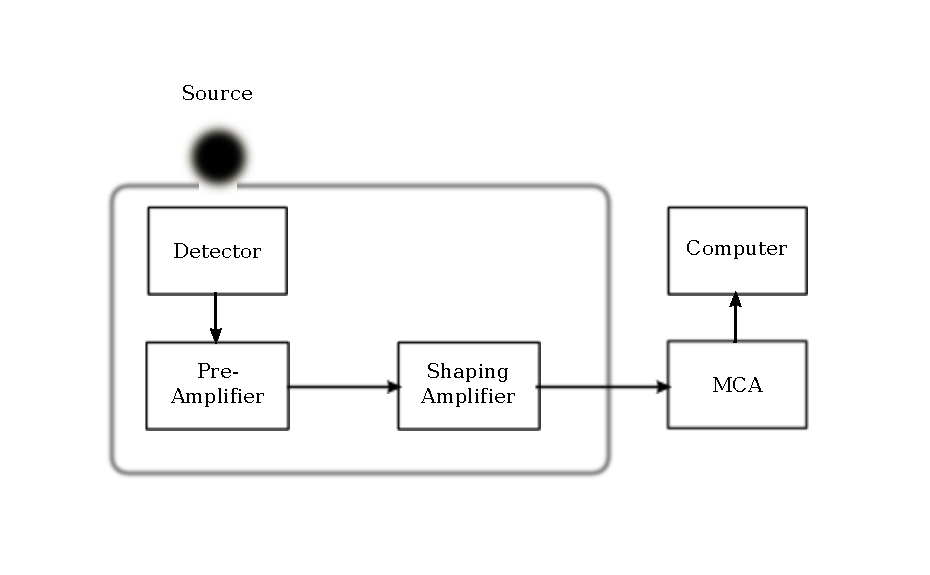
\includegraphics[width=\textwidth]{figures/setup_detector}
    \caption{
        Units for processing the signal of the semiconductor detector.
        Detector, preamplifier and shaping amplifier are located in 
        a box to reduce the background. 
        }
    \label{fig:setup_detector}
\end{figure}


Eval
For the evaluation, we measure each sample with the two detectors for 
one hour each. The calibration of the histogram to actual energies is 
done with the known peaks of $^{57}$Co at $122.06\,$keV and $136.47\,$keV 
as well as the $59.5\,$keV peak of $^{241}$Am. The peaks are fitted on 
gaussians of the form \eqref{eq:gaussian}, and the centers $x_c$ are 
plotted over the corresponding energies $E$. The three points 
are interpolated linearly. 
The parameters obtained by the fit are used to compute
the ratio of the absorption probabilities $\mathrm{Abs}(E)$ for each peak 
as well as the relative energy resolution $\mathrm{RER}(E)$.
The correspondence to the fit parameters are~\cite{ver}
\begin{align}
    \frac{\mathrm{Abs_{Si}}(E)}{\mathrm{Abs_{CdTe}}(E)}
    &= \frac{A_\mathrm{Si}(E) / a_\mathrm{Si}}{A_\mathrm{CdTl}(E) / a_\mathrm{CdTl}} \\
    \begin{split}
        \mathrm{RER}(E) &= \frac{\mathrm{FWHM}(E)}{E} \\
                        &= \frac{2 \sqrt{2 \ln 2} \sigma(E)}{E} \\
                        &\approx \frac{2.35 \sigma(E)}{E} .
    \end{split}    
\end{align}
The additional parameters are the active area $a$, in this case 
\begin{align}
    a_\mathrm{Si}   &= 100 \, \mathrm{mm^2} \\
    a_\mathrm{CdTl} &= \,23 \, \mathrm{mm^2} \, ,
\end{align}
and the full width at half maximum $\mathrm{FWHM}$, which 
is related to the standard deviation as indicated above. 
